% WWW table style: three rules, bold headers, reference green highlight.
\subsection{Complete new public-data suite}
\label{app:new-task-full}
The six new tasks are retained as a complete evaluation set. The suite was
motivated by the geometric hypothesis after examining the earlier archive;
it is a follow-up study rather than an independent confirmation of universal
optimizer superiority. A main-text subset is identified by the rule in
Section~\ref{sec:new-public-tasks}; this appendix retains all six tasks and
all methods regardless of their ranking. No unsuccessful run is deleted
after observing its test result.

\begin{table}[htbp]\centering\small
\caption{New-task data and primary metrics. Preprocessing fits the training
split only. Counts are actual prepared examples, not nominal dataset sizes.}
\reviewfit{\begin{tabular}{lrrrl}\toprule {\bfseries Task} & {\bfseries Train} & {\bfseries Validation} & {\bfseries Test} & {\bfseries Primary metric}\\\midrule
20 Newsgroups  &  9051  &  2263  &  7532  &  Macro-F1 $\uparrow$\\
SMS Spam (deduplicated)  &  3612  &  774  &  774  &  Macro-F1 $\uparrow$\\
Adult  &  26048  &  6513  &  16281  &  AUROC $\uparrow$\\
Spambase  &  3220  &  690  &  691  &  AUROC $\uparrow$\\
Optdigits denoising  &  3058  &  765  &  1797  &  Pixel MSE $\downarrow$\\
Optdigits completion  &  3058  &  765  &  1797  &  Missing-pixel MSE $\downarrow$\\
\bottomrule\end{tabular}}\end{table}

\paragraph{Text.}
20 Newsgroups uses the official by-date train/test split through the
scikit-learn loader, with headers, footers and quotes removed
\cite{sklearn20newsdata}. A stratified 20\% of the official training set is
reserved for validation. TF-IDF uses a vocabulary of at most 2048 terms,
minimum document frequency 2, maximum document frequency 0.95, sublinear
term frequency and row normalization; its vocabulary and inverse document
frequencies fit only the training documents. Official test documents,
including empty texts and exact-text overlaps in the released corpus, are
retained and those counts are recorded; exact-text independence is not
asserted. SMS Spam \cite{uci2011sms} removes exact stripped-message duplicates
and conflicting duplicate labels before a stratified 70/15/15 split. It uses
the same TF-IDF parameters. Both text models use a 64-unit ReLU hidden layer,
dropout 0.1, and a linear classifier. Sparse inputs remain sparse in the first
matrix product. Macro-F1, rather than majority-class accuracy, is the primary
selection metric; predictions use the fixed argmax rule.

\paragraph{Structured data.}
Adult \cite{uci1996adult} retains its official test set and reserves 20\% of
its training rows for stratified validation. Continuous features are
standardized with training statistics; categories are training-fitted one-hot
features, unknown categories are ignored and missing categories are explicit.
Spambase \cite{uci1999spambase} uses a stratified 70/15/15 split and training
standardization. Both models have 128 and 64 ReLU units, dropout 0.1 after
the first hidden layer, and two output logits. The primary metric is AUROC;
accuracy, macro-F1 and cross-entropy are retained as secondary diagnostics.

\paragraph{Inverse imaging.}
The Optdigits corpus \cite{uci1998optdigits} preserves its official
writer-disjoint test set, with 20\% of the original training set reserved
for stratified validation. The 64 pixel features are divided by 16. The
denoising task adds independent Gaussian noise with standard deviation 0.3
and clips corrupted inputs to $[0,1]$. The completion task independently
masks half the pixels and concatenates the visibility mask to the input.
Training uses fresh corruptions on every full epoch; validation and testing
use fixed independent corruptions. The encoder--decoder widths are
128--32--128, with tanh hidden activations and sigmoid output. Denoising
optimizes all-pixel MSE. Completion optimizes missing-pixel MSE; observed
pixels are copied when computing full-image reconstruction MSE and PSNR.
The two tasks do not constitute separate independent image datasets.

\paragraph{Search and state accounting.}
Ranks start at 8 and are capped below the input dimension and at half the
output dimension. Small matrices and biases use full Adam fallback in routed
methods. All weight decays are zero. AdamW searches learning rates
$\{0.0003,0.0005,0.001,0.002,0.003,0.005,0.01,0.02,0.03\}$;
SGD-M searches nine geometrically spaced rates from $0.001$ to 3, with
momentum 0.9. Routed methods cross rates $\{0.001,0.003,0.01\}$ with
residual-rate ratios $\{1,10,100\}$. GrassRoute tracking rates
$\{0.3,1,3\}$ and periodic intervals $\{5,25,100\}$ are assigned in a
balanced cyclic design across those nine cells, not exhaustively crossed.
Official SubTrack++ crosses the same three parameter rates with initial
subspace steps $\{0.1,1,3\}$ and uses the device-only CPU adapter described
above. Adaptive moments use $\beta_1=0.9,\beta_2=0.999$; GrassRoute uses
routing momentum 0.9 and diagonal transport. Fixed and periodic comparators
retain no unused routing momentum. Thin SVD uses a double-precision retry
only if its single-precision decomposition raises a linear algebra error.
Persistent state is measured from allocated optimizer storage, including the
official projector state. Shared-host CPU wall times are not isolated speed
measurements.

All screening runs use 200 complete epochs; final validation selects a
configuration, which is retrained afresh for 1000 epochs before a single
held-out test evaluation. Optimizer random initialization is isolated from
dropout/corruption streams. Restartable checkpoints retain model, optimizer
and random states. Every candidate, numerical failure, full trajectory,
source hash and endpoint remains in the ledger. The frozen manifest is
\path{revision/newtask_results/protocol.json}; the checked outcome ledger is
\path{revision/newtask_status.json}. These new runs do not inflate the
original 162-comparison completion count.

% WWW table style: three rules, bold headers, reference green highlight.
\begin{table}[htbp]\centering\scriptsize\setlength{\tabcolsep}{3pt}
\caption{Complete frozen new-task matrix, seed 42. Nine 200-epoch validation candidates per method, followed by 1000 fresh full epochs. Macro-F1 and AUROC are percentages; image tasks report MSE (missing pixels for inpainting). -- means unfinished or numerically failed, with failures retained in the ledger. Best endpoints are bold only after all six methods complete.}
\label{tab:newtasks-full}
\reviewfit{\begin{tabular}{llrrrrrr}\toprule {\bfseries Task} & {\bfseries Metric} & {\bfseries SGD-M} & {\bfseries AdamW} & {\bfseries Fixed} & {\bfseries Thin SVD} & \cellcolor{oursbg}{\bfseries GrassRoute} & {\bfseries SubTrack++}\\\midrule
Optdigits / denoising  &  MSE $\downarrow$  &  0.0236  &  0.0187  &  0.0325  &  0.0241  &  \cellcolor{oursbg}0.0249 &  \textbf{0.0178}\\
Optdigits / inpainting  &  MSE $\downarrow$  &  0.0412  &  \textbf{0.0296}  &  0.0507  &  0.0379  &  \cellcolor{oursbg}0.0429 &  0.0314\\
Spambase / MLP  &  AUC $\uparrow$  &  \textbf{97.87}  &  97.62  &  97.41  &  97.58  &  \cellcolor{oursbg}97.55 &  97.80\\
Adult / MLP  &  AUC $\uparrow$  &  89.29  &  88.91  &  90.75  &  \textbf{91.23}  &  \cellcolor{oursbg}90.27 &  89.14\\
SMS / TF-IDF MLP  &  F1 $\uparrow$  &  \textbf{95.48}  &  \textbf{95.48}  &  46.69  &  94.29  &  \cellcolor{oursbg}94.63 &  95.40\\
20 News / TF-IDF MLP  &  F1 $\uparrow$  &  \textbf{54.33}  &  50.95  &  52.96  &  53.49  &  \cellcolor{oursbg}52.31 &  50.38\\
\bottomrule\end{tabular}}\end{table}

% WWW table style: three rules, bold headers, reference green highlight.
{\scriptsize\setlength{\tabcolsep}{3pt}
\begin{longtable}{llrrrrr}
\caption{All classification secondary endpoints and state costs in the new suite. Text configurations were selected by macro-F1 and tabular configurations by AUROC, never by the secondary test metrics. Accuracy, F1 and AUC are percentages; cross-entropy is unscaled; persistent state is decimal MB. -- means unfinished or inapplicable.}\label{tab:newtasks-secondary}\\
\toprule {\bfseries Task} & {\bfseries Method} & {\bfseries Accuracy} & {\bfseries Macro-F1} & {\bfseries AUROC} & {\bfseries CE} & {\bfseries State MB}\\\midrule\endfirsthead
\toprule {\bfseries Task} & {\bfseries Method} & {\bfseries Accuracy} & {\bfseries Macro-F1} & {\bfseries AUROC} & {\bfseries CE} & {\bfseries State MB}\\\midrule\endhead
Spambase / MLP & SGD-M & 93.34 & 93.02 & 97.87 & 0.3269 & 0.063\\
Spambase / MLP & AdamW & 94.07 & 93.76 & 97.62 & 0.5338 & 0.127\\
Spambase / MLP & Fixed & 94.07 & 93.78 & 97.41 & 0.4692 & 0.021\\
Spambase / MLP & Thin SVD & 93.63 & 93.34 & 97.58 & 0.3465 & 0.021\\
\rowcolor{oursbg}Spambase / MLP & \textbf{GrassRoute} & 92.19 & 91.81 & 97.55 & 0.3459 & 0.027\\
Spambase / MLP & SubTrack++ & 93.34 & 93.02 & 97.80 & 0.4853 & 0.056\\
Adult / MLP & SGD-M & 84.15 & 77.23 & 89.29 & 0.4159 & 0.089\\
Adult / MLP & AdamW & 84.14 & 76.98 & 88.91 & 0.3993 & 0.179\\
Adult / MLP & Fixed & 85.25 & 78.59 & 90.75 & 0.3185 & 0.022\\
Adult / MLP & Thin SVD & 85.58 & 79.16 & 91.23 & 0.3067 & 0.022\\
\rowcolor{oursbg}Adult / MLP & \textbf{GrassRoute} & 84.86 & 78.31 & 90.27 & 0.3408 & 0.030\\
Adult / MLP & SubTrack++ & 83.71 & 76.94 & 89.14 & 0.4541 & 0.093\\
SMS / TF-IDF MLP & SGD-M & 98.06 & 95.48 & 99.30 & 0.0799 & 0.525\\
SMS / TF-IDF MLP & AdamW & 98.06 & 95.48 & 98.28 & 0.1752 & 1.050\\
SMS / TF-IDF MLP & Fixed & 87.60 & 46.69 & 64.97 & 0.3601 & 0.071\\
SMS / TF-IDF MLP & Thin SVD & 97.67 & 94.29 & 99.02 & 0.0952 & 0.071\\
\rowcolor{oursbg}SMS / TF-IDF MLP & \textbf{GrassRoute} & 97.80 & 94.63 & 99.08 & 0.0931 & 0.137\\
SMS / TF-IDF MLP & SubTrack++ & 98.06 & 95.40 & 97.50 & 0.1415 & 0.153\\
20 News / TF-IDF MLP & SGD-M & 55.12 & 54.33 & -- & 2.1272 & 0.530\\
20 News / TF-IDF MLP & AdamW & 51.66 & 50.95 & -- & 2.4000 & 1.060\\
20 News / TF-IDF MLP & Fixed & 54.25 & 52.96 & -- & 1.4909 & 0.074\\
20 News / TF-IDF MLP & Thin SVD & 54.30 & 53.49 & -- & 1.6752 & 0.074\\
\rowcolor{oursbg}20 News / TF-IDF MLP & \textbf{GrassRoute} & 53.21 & 52.31 & -- & 1.7997 & 0.141\\
20 News / TF-IDF MLP & SubTrack++ & 50.94 & 50.38 & -- & 5.9154 & 0.159\\
\bottomrule\end{longtable}
}

\clearpage
\begin{figure}[htbp]\centering
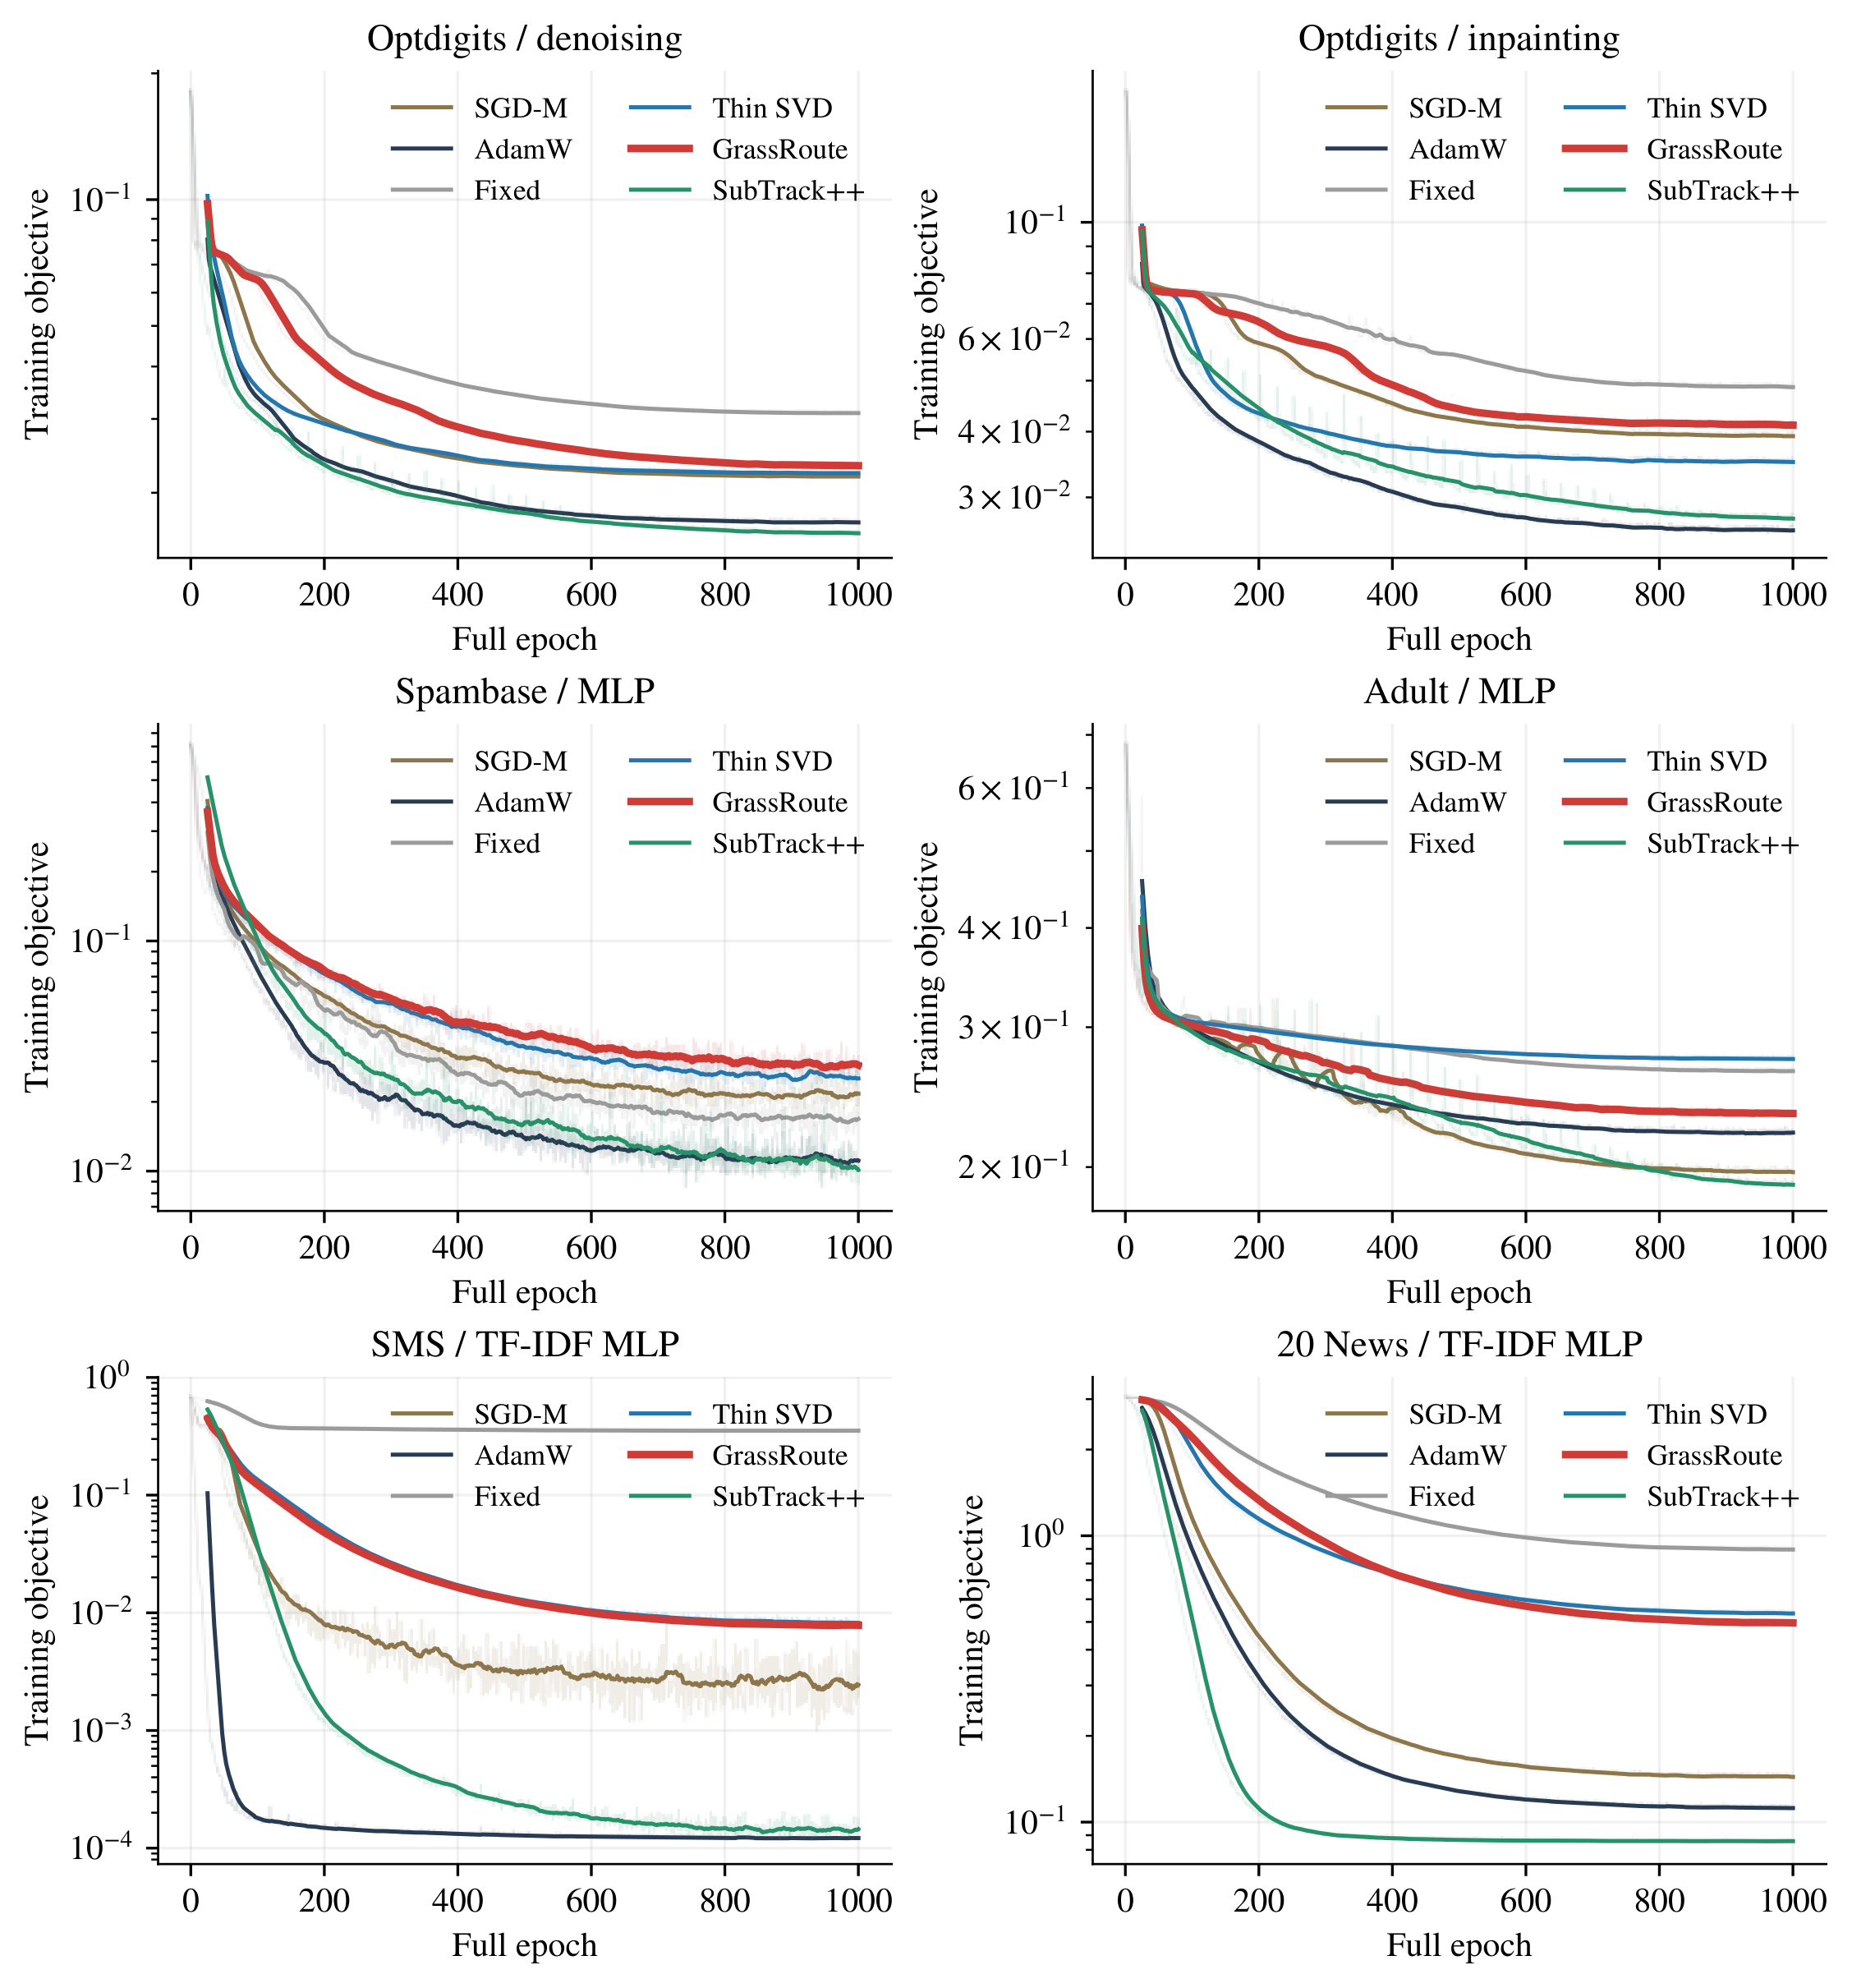
\includegraphics[width=\linewidth]{figures/fig_newtask_losses_all.png}
\caption{Complete new-task training-loss matrix, including every completed
formal optimizer run. Missing curves indicate unfinished or failed formal
training, never an omitted unfavorable endpoint. All full runs have 1000
epochs. Faint lines are raw objectives and solid lines are 25-epoch trailing
means. Task selection for the main-text illustration does not remove any
curve from this complete matrix.}
\label{fig:newtasks-all}
\end{figure}
